% ----------------------------------------------------------
% ------------------- Document preamble --------------------
% ----------------------------------------------------------
\documentclass[11pt,a4paper,openright]{report}

\pdfoutput=1

\usepackage[utf8]{inputenc}
\usepackage{fullpage}
\usepackage{ETHhead3}
\usepackage{url} 
\usepackage{tikz}
\usepackage[intlimits]{amsmath}
\usepackage{bbm}
\usepackage{graphicx}
\usepackage{paralist}
\usepackage[sc]{mathpazo}
\usepackage[english]{babel}
\usepackage{csquotes}
\usepackage[backend=biber,style=alphabetic,sorting=nyt]{biblatex}
\usepackage{fancyref}
\usepackage{hyperref}
\usepackage{booktabs}
\usepackage{appendix}
\usepackage{siunitx}

\addbibresource{thesis.bib}

\hypersetup{colorlinks,citecolor=blue}
\hbadness=3000

% Title page custom commands
\newcommand{\thesistype}[1]{\def\thesistype{#1}}
\newcommand{\advisors}[1]{\def\advisors{#1}}
\newcommand{\department}[1]{\def\department{#1}}

\newcommand{\etal}{\textit{et al.}}

\input{vmr-symbols-vecbold.tex} % Vectors/matrices symbols
\input{standard-macros.tex}     % Common macros

\begin{document}

% ----------------------------------------------------------
% ------------------- Title page ---------------------------
% ----------------------------------------------------------
\title{Tracking Data and Tactical Diagrams in Football}
\thesistype{Master Thesis}
\advisors{Supervisors:\\
		Ulrik Brandes\\
		Hugo Fabrègues\\[5mm]}
\date{August 2025}

\begin{titlepage}
    \ETHhead{Department of Humanities, Social and Political Sciences}{Prof. Dr. U. Brandes}	
    \centering
    \strut\vspace{4cm}
    {\fontsize{25pt}{29pt}\selectfont Master Thesis \\[6mm]
    Thomas Gence\\[10mm]}
    \vspace{2cm}
    {\fontsize{30pt}{34pt}\selectfont \bfseries Tracking Data and Tactical Diagrams in Football \par}
    \vspace{3cm}
    {\fontsize{18pt}{22pt}\selectfont \advisors \par}
    \vspace{0.5cm}
    {\fontsize{16pt}{20pt}\selectfont August 2025 \par} 
    \vfill
\end{titlepage}

\newpage
\pagenumbering{roman}

% ----------------------------------------------------------
% ------------------- Abstract -----------------------------
% ----------------------------------------------------------
\chapter*{Abstract}
\addcontentsline{toc}{chapter}{Abstract}
Football analytics has entered a new era thanks to detailed event and tracking data, yet the translation of these raw datasets into actionable tactical insights remains a challenge for both practitioners and researchers. Current visualization tools are either overly manual, lack standardization, or provide poor integration with match data. This thesis proposes a comprehensive system of requirements, interaction models, and a standardized visual language for the next generation of tactical diagramming platforms in football. Building on the analysis of existing software and research literature, we set out a conceptual and practical framework for creating, annotating, and comparing tactical diagrams—both manually and from data. The primary contribution is not a finished application, but a design blueprint for future tool development, aiming to close the gap between data science and coaching practice.

% ----------------------------------------------------------
% ------------------- Acknowledgments ----------------------
% ----------------------------------------------------------
\chapter*{Acknowledgments}
\addcontentsline{toc}{chapter}{Acknowledgments}
My sincere thanks to my supervisors Prof. Ulrik Brandes and Hugo Fabrègues for their guidance and support. Special appreciation goes to my family and friends for their continuous encouragement throughout my studies.

% ----------------------------------------------------------
% ------------------- Table of Contents --------------------
% ----------------------------------------------------------
\tableofcontents

% ----------------------------------------------------------
% ------------------- Notation -----------------------------
% ----------------------------------------------------------
\chapter*{Notation}
\addcontentsline{toc}{chapter}{Notation}

% (Add symbols, abbreviations, pitch dimensions, etc.)

% ----------------------------------------------------------
% ------------------- Introduction -------------------------
% ----------------------------------------------------------
\chapter{Introduction}
\pagenumbering{arabic}
Football is widely recognized as the most popular sport globally, with a rich history of tactical innovation and analysis. In recent years, the discipline of football analytics has expanded dramatically, driven by advances in data collection, processing, and visualization. Clubs, coaches, and analysts now routinely leverage event and tracking data to inform match preparation, tactical training, and performance evaluation \cite{sarmento2014match, perin2013soccerstories}. 

Yet, while access to data has never been greater, the process of turning raw positional and event information into actionable tactical knowledge remains challenging. Analysts and coaches still rely heavily on manual diagramming—on whiteboards, paper, or basic digital tools—to communicate ideas about formations, player roles, and movement. Even when data-driven models (e.g., xG, pitch control) are available, their visual outputs are often too technical or inflexible for day-to-day coaching or match analysis sessions \cite{sacha2014feature, perin2013soccerstories}.

A central gap in current practice is the lack of standardized, interactive, and data-integrated visual languages for tactical communication. Many commercial products offer basic pitch drawing features, but rarely support seamless integration of tracking/event data, and their visual conventions (arrows, colors, player symbols) lack theoretical grounding or standardization. This gap is reflected in recent calls from both research and practice for systems that can bridge the divide between data science and the everyday needs of coaches \cite{maiden2023designing, perin2013soccerstories}.\\


\textbf{Aims and Scope.}  
\\\\
This thesis aims to provide a blueprint for such a system by:
\begin{itemize}
    \item Reviewing the state of the art in football data and tactical diagramming tools.
    \item Formalizing the requirements (user, functional, and visual) for a next-generation tactical analysis platform, grounded in literature and expert review.
    \item Designing a visual language and data architecture for flexible, coach-friendly, and data-driven diagramming.
    \item Providing prototyping guidelines and use cases to facilitate future tool development.
\end{itemize}
By focusing on the design and requirements level—rather than delivering a finished application—this work addresses a critical need at the intersection of sports analytics, human-computer interaction, and coaching practice.

% ----------------------------------------------------------
% ------------------- Background ---------------------------
% ----------------------------------------------------------
\chapter{Background and Related Work}
\label{chap:context}

% ------------------- Football Data: Event and Tracking Systems -----------------------
\section*{Football Data: Event and Tracking Systems}
The digital transformation of football analytics has been driven by the proliferation of large, structured datasets, enabled by technological advances in data capture and storage \cite{morgulev2018sports}. Two data types are now fundamental:

\begin{itemize}
    \item \textbf{Event data}: Sequences of time-stamped football actions (passes, shots, tackles), collected by major data providers (Opta, Wyscout, StatsBomb). Event data is the basis for traditional match statistics, advanced possession metrics, and models like Expected Goals (xG) or Expected Threat (xT) \cite{sarmento2014match}. These event logs are standardized, but their real tactical value is only revealed when connected to the evolving spatial structure of play.
    \item \textbf{Tracking data}: Leveraging optical tracking or GPS technology, modern systems (TRACAB, Second Spectrum) capture XY coordinates of all players and the ball, often at 10–25 Hz, throughout matches \cite{sacha2014feature}. This granular data enables dynamic analyses: team shape, pressing behavior, spatial dominance, and player workloads \cite{morgulev2018sports}. However, aligning these continuous spatial streams with the episodic, conceptual language of tactics remains an ongoing challenge.
\end{itemize}

Crucially, these two data streams have different temporal, semantic, and representational structures—posing significant challenges for integration into a unified tactical analysis framework \cite{sarmento2014match, perin2013soccerstories}. Mapping raw data to diagrams that reflect expert tactical understanding remains a partly manual, interpretive process, as highlighted in both academic and applied literature.

% ------------------- Tactical Diagrams: Practice and Visualization Challenges -------
\section*{Tactical Diagrams: Practice and Visualization Challenges}
Tactical diagrams are the lingua franca of football coaching. Coaches and analysts rely on hand-drawn or digitally sketched diagrams to communicate everything from base formations to sophisticated movement patterns and pressing triggers \cite{maiden2023designing, perin2013soccerstories}. However, three persistent issues emerge:

\begin{itemize}
    \item \textbf{Lack of standardization}: There is no universally agreed-upon notation for diagramming football tactics. As Perin et al.\ document in \textit{SoccerStories} \cite{perin2013soccerstories}, existing tools and media use ad hoc combinations of arrows, icons, and colors, resulting in inefficiencies and confusion, especially in collaborative or educational contexts.
    \item \textbf{Data integration barriers}: Although clubs now possess vast datasets, the process of turning raw event/tracking data into tactical diagrams is rarely automated. Most diagrams are still static, hand-crafted images, sometimes annotated screenshots, with little or no dynamic linkage to underlying match data \cite{sarmento2014match, perin2013soccerstories}. SoccerStories found that even expert analysts and journalists often relied on manual sketches, heatmaps, or simple tables to convey tactical stories, despite having access to richer data streams.
    \item \textbf{Limited interactivity and usability}: Most digital tools (TacticalPad, KlipDraw, Hudl) prioritize drawing features over truly interactive exploration. As Perin et al.\ and others highlight, coaches value rapid, touch-based exploration and side-by-side comparison, but few tools provide synchronized, interactive environments for hypothesis testing or real-time scenario analysis \cite{perin2013soccerstories, maiden2023designing}.
\end{itemize}

Qualitative studies \cite{perin2013soccerstories} show that experts desire tools that support both exploratory analysis and effective communication (“telling stories”), combining robust statistical underpinnings with intuitive, context-rich visuals. This thesis is thus positioned at the intersection of these needs—seeking to formalize and standardize the mapping between data and visual tactical language.

% ------------------- Lessons from SoccerStories and Feature-Driven Visual Analytics --
\section*{Lessons from SoccerStories and Feature-Driven Visual Analytics}
A key milestone in the scientific literature is the SoccerStories project by Perin et al.\ \cite{perin2013soccerstories}, which developed an exploratory visualization environment that organizes match data by “phases” (sequences of actions with common tactical meaning), using faceted views tailored for specific events (passes, shots, runs). User studies found that analysts and journalists value:
\begin{itemize}
    \item Overviews and timelines to identify phases of interest;
    \item Linked visualizations (e.g., node-link diagrams, heatmaps) that provide multi-layered context;
    \item The ability to compare planned (theoretical) and actual (executed) player positions and movements.
\end{itemize}
SoccerStories’ approach to structuring data visually, and its evaluation with real practitioners, provide methodological inspiration for this design blueprint.

Further, recent works like Sacha et al.'s “Feature-Driven Visual Analytics of Soccer Data” \cite{sacha2014feature} show the value of combining event data with spatiotemporal visualizations, supporting both “overview first, zoom and filter, then details-on-demand” paradigms. The consensus in the literature is that tools must bridge the “last mile” between data science and coaching practice, by grounding design decisions in actual analyst workflows.

% ------------------- Requirements Engineering in Sports Analytics: Scientific Justification --
\section*{Requirements Engineering in Sports Analytics: Scientific Justification}
A robust requirements engineering process is essential for developing useful sports analytics tools. As discussed in Morgulev et al.\ \cite{morgulev2018sports} and Maiden et al.\ \cite{maiden2023designing}, user-centered design should begin with:
\begin{itemize}
    \item \textbf{Task analysis}: Identifying the real-world scenarios where coaches and analysts use diagrams (e.g., halftime adjustments, training drills, post-match review).
    \item \textbf{Stakeholder interviews}: Engaging both end-users (coaches, analysts, technical staff) and organizational decision-makers.
    \item \textbf{Iterative prototyping}: Testing early versions of tools through scenario-based walkthroughs, direct feedback, and competitive benchmarking.
    \item \textbf{Context constraints}: Recognizing the importance of tablet/touchscreen interaction, fast switching between diagram modes, and limited available time for analysis.
\end{itemize}
Such a methodology is now considered best practice in the development of domain-specific analytics platforms.

% ------------------- Gaps and Research Opportunities ---------------------
\section*{Gaps and Research Opportunities}
While many commercial platforms claim “data-driven” tactical analysis, the academic literature and recent reviews (e.g., Sarmento et al.\ \cite{sarmento2014match}) agree that integration of tracking/event data into truly interactive, interpretable visual environments remains a key research frontier. This thesis directly addresses this need, proposing a requirements-driven design blueprint that draws on both competitive analysis and expert validation. The expectation, as also articulated in SoccerStories \cite{perin2013soccerstories}, is that future tools must “close the gap between data science and coaching practice” by enabling intuitive, standardized, and evidence-based diagramming.

% ----------------------------------------------------------
% ------------------- Contribution and Scope ---------------
% ----------------------------------------------------------
\chapter{Contribution and Scope}
This thesis delivers:
\begin{itemize}
    \item A detailed, structured list of system and user requirements, informed by competitive analysis and literature.
    \item A standardized visual language for tactical diagrams, developed through analysis of existing tools and best practices.
    \item Workflows for diagram creation, annotation, and interactive manipulation, tailored to touch devices.
    \item Prototyping layouts and case scenarios to guide future software implementation.
\end{itemize}
Crucially, this work is a design and planning blueprint—not a finished product—and emphasizes the translation of complex data into usable, interpretable, and pedagogically effective visual forms.

% ----------------------------------------------------------
% ------------------- Methodology (Expanded) ---------------
% ----------------------------------------------------------

\chapter{Methodology}
\section{Overview and Rationale}

The methodology for this thesis is grounded in design research, combining comparative analysis of existing tools, an iterative approach to defining requirements, and the application of visualization theory. Given the limited literature on the standardization of football diagramming, much of the process was necessarily exploratory and based on best practices in the visualization field, complemented by domain expertise in sports analytics. This chapter transparently details the methods and justifications for each design choice.


\section{Design Process and Sources}

\subsection{Literature Review and Market Analysis}

The initial phase involved a literature review focusing on football analytics, visualization standards, and user needs in sports analysis. Key references include Perin et al.\ \cite{perin2013soccerstories}, Sarmento et al.\ \cite{sarmento2014match}, and Sacha et al.\ \cite{sacha2014feature}, who highlight the lack of standardized visual language and the prevalence of ad hoc conventions in existing tools. In parallel, a market analysis of commercial products (e.g., TacticalPad, KlipDraw, Hudl) and research prototypes (e.g., SoccerStories, motion chart tools) was conducted to identify common features, gaps, and interface patterns.

\subsection{Comparative and Heuristic Analysis}

Rather than applying a single formal method, the process relied on comparative/heuristic analysis---an established approach in HCI and visualization research when empirical user studies are not feasible \cite{munzner2014visualization}. The aim was to identify (a) core requirements recurring across tools and literature; (b) best practices or pitfalls in the representation of football actions; and (c) opportunities for improvement in interactivity and data integration.

\subsection{Expert Feedback and Iterative Refinement}

Design iterations incorporated domain expertise and practical knowledge of coaching workflows and analysis conventions, with a focus on ergonomic principles and alignment with the available literature. For example, the choice of a vertical pitch orientation and clear player/role encoding draws from cognitive ergonomics and perceptual best practices (see e.g., \cite{perin2013soccerstories, munzner2014visualization}). Where scientific references were unavailable, decisions are supported by conventions observed in professional football analysis tools.


\section{Requirements Elicitation}

Requirements were synthesized by triangulating three sources:
\begin{enumerate}
\item \textbf{Literature and competitive analysis:} Documenting functional needs and interface patterns (see Table~\ref{tab:requirements}).
\item \textbf{Own experience:} As a user of both commercial and academic tools, and from practical prototyping with Figma and Lucidchart.
\item \textbf{Supervisor input:} Regular feedback loops with supervisors ensured alignment with real-world analysis needs and research priorities.
\end{enumerate}

This approach follows best practices in requirements engineering for sports analytics \cite{maiden2023designing, morgulev2018sports}, though with the limitation that no structured interviews or field studies with professional coaches were conducted.

\section{Visual Language Definition}

\subsection{Derivation of Visual Conventions}

The definition of the visual language followed two main steps:
\begin{itemize}
\item \textbf{Comparative synthesis:} Collating conventions from the scientific literature, commercial toolkits, and practical usage in coaching contexts.
\item \textbf{Theoretical grounding:} Justifying choices with established visualization theory—for example, using arrows for directionality and motion \cite{ware2013information, bertin2011semiology}, color coding for categorical distinction \cite{munzner2014visualization}, and a vertical pitch orientation to enhance perceptual congruence with football-specific spatial cognition \cite{perin2013soccerstories}.
\end{itemize}


Where possible, conventions align with upcoming standards (such as FIFA’s EPTS data formats), even if visual standards per se are not yet published by FIFA~\cite{fifa2024epts}. The visual language remains intentionally extensible, allowing adaptation to future research or practical findings.

\subsection{Justification of Specific Choices}

Examples:
\begin{itemize}
\item \textbf{Passes and runs:} Solid arrows are used for passes/dribbles, in line with both common software and recommendations from perception research~\cite{ware2013information, bertin2011semiology}.
\item \textbf{Player tokens:} Circles with color/number are retained for maximal recognizability and minimal cognitive load~\cite{perin2013soccerstories, metulini2016spatio}.
\item \textbf{Pitch orientation:} The pitch is oriented vertically to match player spatial cognition and common practice in tactical analysis tools \cite{perin2013soccerstories, munzner2014visualization}.

\end{itemize}

\subsection{Limitations}

The methodology did not include empirical validation with external end-users. As recommended in HCI and visualization research~\cite{maiden2023designing, munzner2014visualization}, future work should assess the usability and effectiveness of these visual conventions through studies involving professional analysts and coaches, using empirical protocols such as user studies or interviews.


\section{Tools and Prototyping}

The visual language and interaction flows were prototyped in Figma and Lucidchart. For future work, a coding pipeline (e.g., using Python, D3.js, or a dedicated LaTeX package) is planned for direct conversion from tracking data to standardized diagrams. However, the core of this thesis remains at the design/requirements stage.




% ------------------- Development of a Standardized Visual Language (Expanded) -----
\chapter{Development of a Standardized Visual Language}
\label{chap:visual_language}

The effectiveness of tactical diagrams in football is intrinsically linked to the clarity, consistency, and standardization of their visual language---that is, the conventions and graphical elements used to encode tactical information. This chapter reviews the rationale behind the chosen visual conventions, referencing both established visualization theory and domain-specific practices in sports analytics.

\section{The Need for Standardized Notation in Football Tactics}
Despite the centrality of tactical diagrams in football, there is \textit{no universally agreed-upon visual language} for representing formations, movements, and key events. Perin et al.\ \cite{perin2013soccerstories} emphasize that ``the lack of standard visual conventions makes diagrams difficult to interpret, especially in collaborative and educational contexts.'' Most commercial and academic tools rely on ad hoc combinations of arrows, glyphs, and color codes, which, while familiar to their users, hinder communication and reproducibility \cite{sarmento2014match, perin2013soccerstories}.

\section{Principles from Visualization Theory}
Visualization researchers have long argued for the importance of consistent graphical conventions. According to Munzner~\cite{munzner2014visualization}, ``the effectiveness of a visual representation depends on the conventions adopted and their consistency with user expectations and domain standards.'' Bertin~\cite{bertin2011semiology} further argues that conventions, while sometimes arbitrary at first, become powerful tools for communication when shared and widely adopted.

Aigner et al.\ \cite{aigner2007visualizing} highlight that standardization of glyphs and visual markers is essential for comparing complex, time-oriented data. Ware~\cite{ware2013information} shows that intuitive and domain-relevant encodings---for example, using arrows to indicate directionality or dashed lines for hypothetical actions---reduce cognitive load and enhance interpretation.

\section{Adapting and Justifying Visual Conventions for Football}
Most visual languages in football analytics converge on a small set of conventions:
\begin{itemize}
    \item \textbf{Arrows}: Used to indicate player movement, passes, and runs. Typically, solid arrows represent on-ball actions, while dashed or curved arrows can represent off-ball movement or hypothetical alternatives.
    \item \textbf{Colored tokens}: Players are depicted as colored circles or icons, with color encoding team or positional role \cite{perin2013soccerstories, metulini2016spatio}.
    \item \textbf{Field geometry}: The pitch is shown to scale, with half-spaces and zones sometimes overlaid for spatial context.
    \item \textbf{Temporal markers}: When visualizing sequences, frame indices (e.g., 1/3, 2/3) or color gradients are used to show progression through time \cite{sacha2014feature, aigner2007visualizing}.
\end{itemize}

The conventions selected in this thesis are justified as follows:
\begin{itemize}
    \item \textbf{Alignment with user expectations}: We adopt conventions that are already familiar to coaches and analysts, following the principle of ``least surprise''~\cite{munzner2014visualization}.
    \item \textbf{Consistency with domain standards}: Where possible, the design aligns with FIFA's emerging documentation for football data visualization.
    \item \textbf{Support from the literature}: Visualization theory consistently emphasizes the benefits of standardization, both for learning and for collaborative analysis~\cite{bertin2011semiology, ware2013information}.
    \item \textbf{Extensibility}: The language is designed to be extensible, allowing new conventions (e.g., for new metrics or roles) to be incorporated without undermining overall consistency.
\end{itemize}

As Metulini~\cite{metulini2016spatio} and Perin et al.~\cite{perin2013soccerstories} both highlight, a standardized, well-justified visual language is not only a technical convenience but a prerequisite for effective communication and knowledge transfer in sports analytics.

\section{Visual Language Reference Table}

\begin{center}
\textbf{\Huge Visual Language Reference}
\end{center}

\vspace{0.5cm}
\begin{itemize}
    \item \textbf{Players:}
    \begin{itemize}
        \item \textbf{Strategy View:}
        \begin{itemize}
            \item 
            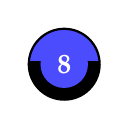
\begin{tikzpicture}[scale=0.45,baseline=-0.6ex]
                \begin{scope}
                    \clip (0,0) circle (1);
                    \fill[black] (-1,-1) rectangle (1,0.1);
                    \fill[blue!70] (-1,0.1) rectangle (1,1);
                \end{scope}
                \fill[blue!70] (0,0) circle (0.67);
                \draw[thick] (0,0) circle (1);
                \node[white] at (0,0) {\textbf{8}};
            \end{tikzpicture}
            \quad Upside color (T-shirt) / Downside color (Shorts)
        \end{itemize}
        \item \textbf{Tactics View:}
        \begin{itemize}
            \item \textbf{Home Team (Attacker):}
            \begin{itemize}
                 \item 
                 
\begin{tikzpicture}[scale=0.45,baseline=-0.6ex]
                \draw[red, thick] (0,0) circle (0.6);
                \end{tikzpicture}
                \quad Attacker (non-ball carrier)
                \item 
                
\begin{tikzpicture}[scale=0.45,baseline=-0.6ex]
                \draw[very thick, red] (0,0) circle (0.8);
                \draw[red, thick] (0,0) circle (0.6);
                \end{tikzpicture}
                \quad Ball carrier
            \end{itemize}
            \item \textbf{Away Team (Defender):}
            \begin{itemize}
            \item 
            
\begin{tikzpicture}[scale=0.5,baseline=-0.6ex]
                \node[blue, thick] at (0,0) {\Huge $\times$};
            \end{tikzpicture}
            \quad Defender
            \end{itemize}
        \end{itemize}
    \end{itemize}
    \item \textbf{Arrow Types:}
    \begin{itemize}
        \item 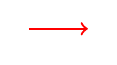
\begin{tikzpicture}[scale=0.5,baseline=-0.6ex]
            \draw[->, thick, red] (0,0) -- (1.5,0);
        \end{tikzpicture}
        \quad Pass
        \item 
\begin{tikzpicture}[scale=0.5,baseline=-0.6ex]
            \draw[->, thick, red, decorate, decoration={snake, amplitude=1.5}] (0,0) -- (1.5,0);
        \end{tikzpicture}
        \quad Dribble
        \item \begin{tikzpicture}[scale=0.5,baseline=-0.6ex]
            \draw[->, thick, red, dashed] (0,0) -- (1.5,0);
        \end{tikzpicture}
        \quad Off-ball run
        \item 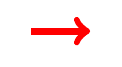
\begin{tikzpicture}[scale=0.5,baseline=-0.6ex]
            \draw[->, line width = 2.5pt, red] (0,0) -- (1.5,0);        
        \end{tikzpicture}
        \quad Shot
        \item \begin{tikzpicture}[scale=0.5,baseline=-0.6ex]
            \draw[->, thick, blue, dashed] (0,0) -- (1.5,0);
        \end{tikzpicture}
        \quad Defensive retreat / Pressing
        \item 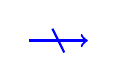
\begin{tikzpicture}[scale=0.5,baseline=-0.6ex]
            \draw[->, thick, blue] (0,0) -- (1.5,0);
            \draw[blue, thick] (0.6,0.3) -- (0.9,-0.3);
        \end{tikzpicture}
        \quad Tackle attempt
    \end{itemize}
    \item \textbf{Special Zones:}
    \begin{itemize}
        \item \begin{tikzpicture}[scale=0.5,baseline=-0.6ex]
            \draw[dashed, gray!70, line width=1pt] (0,0) -- (2.5,0);
        \end{tikzpicture}
        \quad Positional alignment lines
        \item 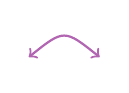
\begin{tikzpicture}[scale=0.45,baseline=-0.6ex]
            \draw[<->, thick, violet!60] (0,0) .. controls (1,0.8) .. (2,0);
        \end{tikzpicture}
        \quad Permutation possibility
        \item 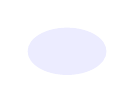
\begin{tikzpicture}[scale=0.5,baseline=-0.6ex]
            \fill[blue!30, opacity=0.25] (0,0) ellipse (1 and 0.6);
        \end{tikzpicture}
        \quad Pressing zone
        \item 
\begin{tikzpicture}[scale=0.5,baseline=-0.6ex]
            \fill[red!30, opacity=0.4] (0,-1) -- (-1,1) -- (1,1) -- cycle;
        \end{tikzpicture}
        \quad Shooting zone
    \end{itemize}
\end{itemize}

\section{Limitations and Open Challenges}
While this thesis adopts a set of conventions grounded in both theory and practice, several open questions remain. For example, how best to represent overlapping events, ambiguity in player roles, or new tactical concepts as the game evolves? Literature from outside football (e.g., in systems biology or process mining) may offer further inspiration~\cite{munzner2014visualization, ware2013information}. Ultimately, as Bertin~\cite{bertin2011semiology} notes, conventions must balance stability and adaptability, evolving with user needs and domain advances.



% ------------------- Mapping Data to Diagrams (Expanded) -------------------------
\chapter{Mapping Data to Diagrams}
\label{chap:data_to_diagram_mapping}

A core challenge in football analytics is not only to design an effective visual language, but also to create a practical workflow for mapping raw tracking and event data into annotated tactical diagrams. This chapter details the system architecture and interfaces enabling the transformation from data to visual representation.

\section{Data Mapping Interfaces}

A dedicated mapping UI allows users to link incoming tracking data (often anonymized or with external IDs) to meaningful squad and formation definitions. This step ensures consistency of player roles and supports scenario-based annotation.

\section{Timeline and Frame Selection}

Inspired by video editing and annotation platforms, timeline controls such as seek bars and frame markers let users navigate to key moments, select sequences, and annotate both individual frames and multi-moment scenarios.

\section{Annotation and Linking Across Sequences}

Annotations are not limited to single frames. Users can link instructions or comments across multiple moments, reflecting the continuity of tactical actions and supporting both micro (frame-level) and macro (sequence-level) analysis.

\section{Best Practices and References}

Future implementers should refer to both the FIFA documentation and current best practices in HCI and sports analytics for effective visual mapping~\cite{maiden2023designing, perin2013soccerstories, sacha2014feature}.





% ----------------------------------------------------------
% ------------------- Implementation (Expanded) ------------
% ----------------------------------------------------------

\chapter{Implementation}

% ------------------- Data Integration and Overlay (Expanded) -----------------
\section{Data Integration and Overlay}

The data integration module is architected to be highly extensible:

Multi-standard support: By default, it expects FIFA-compliant tracking data but can also ingest custom CSV/JSON formats. When a dataset does not match the internal schema, the user is prompted with a mapping UI.

Timeline management: A visual timeline widget enables users to select single frames or define a range (with chosen intervals), which then loads as a sequence of diagrams for annotation and comparison.

Persistence: Each diagram and sequence is saved with metadata (teams, match date, frame indexes), and all user annotations (arrows, text, highlights) are serialized with the diagram state for seamless reloading and future comparison.

% ------------------- Split-Screen, Timeline, and Comparison Features (New Section) -----
\section{Split-Screen, Timeline, and Comparison Features}

A distinguishing feature of the platform is its ability to display and interact with two or more diagrams simultaneously:

Split-screen mode allows users to compare any two diagrams—strategy vs. strategy, or tactical alternatives within the same scenario.

For sequence analysis, a timeline slider enables the user to select which frames appear in each panel, facilitating both “what happened” and “what should have happened” discussions.

Frame index notation (e.g., “1/3, 2/3, 3/3”) appears in each panel, mirroring best practices in professional analysis tools.

Annotations can be created in both panels and even linked, enabling users to highlight differences or suggest alternative actions directly on the interface.

% ----------------------------------------------------------
% ------------------- Conclusion ---------------------------
% ----------------------------------------------------------
\chapter{Conclusion} 
This thesis demonstrates the potential of integrating tracking data with intuitive tactical diagrams, significantly enhancing tactical analyses and decision-making processes in football analytics.

% ----------------------------------------------------------
% ------------------- Bibliography -------------------------
% ----------------------------------------------------------
\clearpage
\printbibliography[heading=bibintoc]

% ----------------------------------------------------------
% ------------------- Appendix -----------------------------
% ----------------------------------------------------------
\appendix
\chapter{List of Requirements} 
A comprehensive list detailing all functional and non-functional requirements as defined throughout the project lifecycle.

% ----------------------------------------------------------
% ------------------- Prototyping Diagrams -----------------
% ----------------------------------------------------------
\chapter{Prototyping Diagrams}

This appendix presents a selection of prototyping screens developed during the thesis. These prototypes illustrate the evolution of the user interface, the visual language for tactical diagrams, and the interaction workflows discussed in the main chapters. Each screenshot below is accompanied by a brief commentary on its purpose, design rationale, and the key requirements it demonstrates.

\section*{A. Strategy Modules: Navigation and Visual Organization}

\textbf{1. Formations Screen}\
\begin{center}
\includegraphics[width=0.7\textwidth]{thesis_latex/Figures/STRATEGY-FORMATIONS.png}
\end{center}
\noindent
This screen allows the user to select, view, and customize team formations. Players are shown in their assigned positions on a scaled pitch, with the formation (e.g., 4-3-3) clearly labeled. The horizontal formation selector at the bottom enables quick switching between preset tactical shapes, while maintaining team color and player role consistency.

\textbf{2. Instructions Screen}\
\begin{center}
\includegraphics[width=0.7\textwidth]{thesis_latex/Figures/STRATEGY-INSTRUCTIONS.png}
\end{center}
\noindent
The “Instructions” module enables coaches to add tactical directions using arrows, curved lines, and freehand annotations. Player tokens remain interactive, and the selected formation is retained as the underlying template.

\textbf{3. Squad Management}\
\begin{center}
\includegraphics[width=0.7\textwidth]{thesis_latex/Figures/STRATEGY-SQUAD.png}
\end{center}
\noindent
Here, the squad list is shown below the pitch, grouped by preferred position. Drag-and-drop is supported for player assignment, and the visual encoding highlights both shirt color and number.

\section*{B. Comparative and Interactive Analysis}

\textbf{4. Split-Screen Comparison}\
\begin{center}
\includegraphics[width=0.8\textwidth]{thesis_latex/Figures/STRATEGY-SPLITSCREEN.png}
\end{center}
\noindent
Split-screen mode supports direct, side-by-side comparison of tactical scenarios. This feature is critical for aligning “planned” vs. “actual” diagrams (e.g., theory vs. match execution), a core requirement identified in both literature and practitioner feedback.

\section*{C. Tactics and Real/Virtual Analysis}

\textbf{5. Tactics: Real Mode}\
\begin{center}
\includegraphics[width=0.8\textwidth]{thesis_latex/Figures/TACTICS-REAL.png}
\end{center}
\noindent
This module overlays tactical annotations on actual match images (video stills or screenshots). The “real” view is used for post-match debriefing, illustrating in-game movement and comparing it to the coach’s plan.

\textbf{6. Tactics: Virtual Mode}\
\begin{center}
\includegraphics[width=0.8\textwidth]{thesis_latex/Figures/TACTICS-VIRTUAL.png}
\end{center}
\noindent
The virtual pitch enables detailed diagramming of hypothetical or alternative tactical phases, independent of video footage. Here, both teams are shown, and player tokens, movements, and key events (passes, runs) can be annotated directly.



\end{document}
